\documentclass[tikz, border=10pt]{standalone}
\usepackage{tkz-graph}
\usepackage{amsmath,amssymb}
\usepackage{xcolor}
\usetikzlibrary{calc}
\usetikzlibrary{positioning}
\usetikzlibrary{shapes}
\usepackage{tikzpeople}

\begin{document}

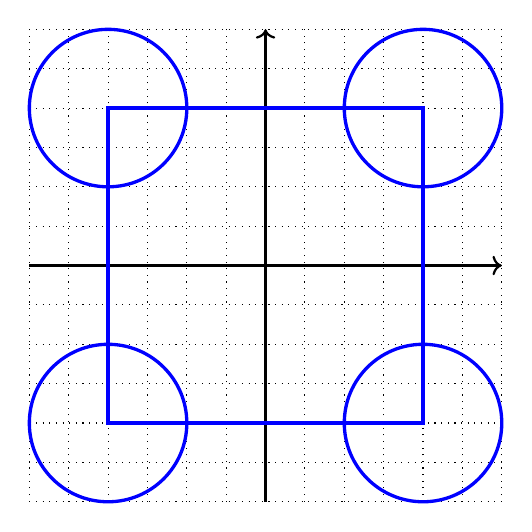
\begin{tikzpicture}
	\draw [thin, dotted, step=0.5] (-3, -3) grid (3,3) ;
	\draw [thick, ->] (-3, 0) -- (3, 0);
	\draw [thick, ->] (0, -3) -- (0, 3);
	\draw [very thick, blue] (-2,-2) -- (-2, 2) -- (2, 2) -- (2, -2) -- cycle;
	\draw [very thick, blue] (-2,-2) circle(1) (-2, 2) circle(1) (2, 2) circle(1) (2, -2) circle(1);
\end{tikzpicture}


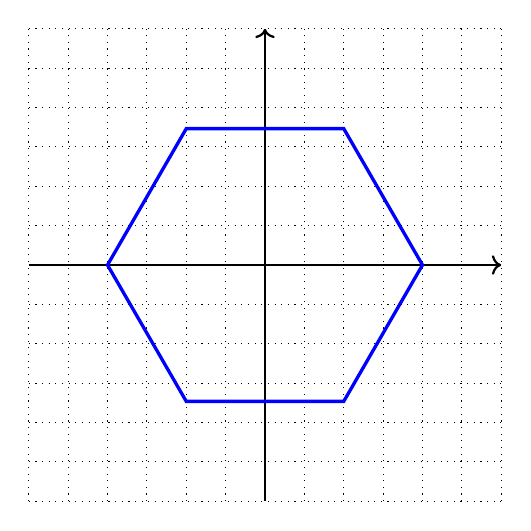
\begin{tikzpicture}
	\draw [thin, dotted, step=0.5] (-3, -3) grid (3,3) ;
	\draw [thick, ->] (-3, 0) -- (3, 0);
	\draw [thick, ->] (0, -3) -- (0, 3);
	\draw [very thick, blue] (0:2) -- (60:2) -- (120:2) -- (180:2) -- (240:2) -- (300:2) -- cycle ;
\end{tikzpicture}



\sffamily
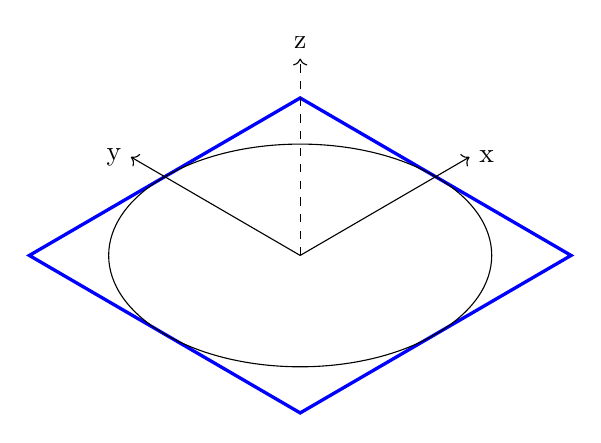
\begin{tikzpicture}[x={(0.86cm,0.5cm)}, y={(-0.86cm,0.5cm)}, z={(0cm,1cm)}]
	\draw[very thick, blue] (-2,-2,0) -- (-2,2,0) -- (2,2,0) -- (2,-2,0) -- cycle;
	\draw[->] (0,0,0) -- (2.5, 0, 0) node [right] {x};
	\draw[->] (0,0,0) -- (0, 2.5, 0) node [left] {y};
	\draw[->,dashed] (0,0,0) -- (0, 0, 2.5) node [above] {z};
	\draw circle (2);

\end{tikzpicture}


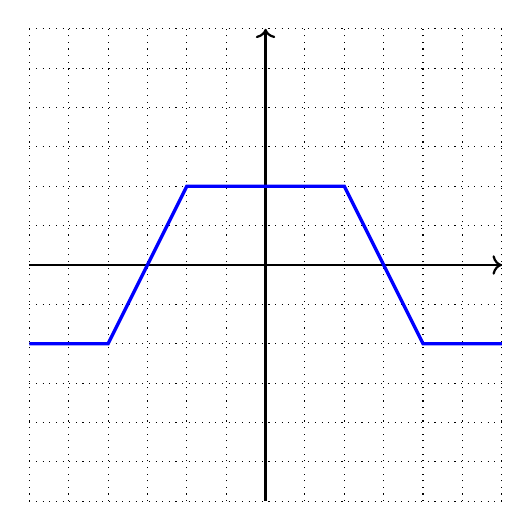
\begin{tikzpicture}
	\draw [thin, dotted, step=0.5] (-3, -3) grid (3,3) ;
	\draw [thick, ->] (-3, 0) -- (3, 0);
	\draw [thick, ->] (0, -3) -- (0, 3);
	\draw [very thick, blue] (-3, -1) -- +(1,0) -- +(2,2) -- +(4,2) -- +(5, 0) -- +(6,0);
\end{tikzpicture}



\begin{tikzpicture}
	\draw[shading=ball, ball color=yellow] (0,0) circle [radius=2];
	\draw[shading=ball, ball color =black] (-0.5, 0.5) ellipse [x radius=0.2, y radius=.4];
	\draw[shading=ball, ball color =black] (0.5, 0.5) ellipse [x radius=0.2, y radius=.4];
	\draw[very thick] (-1,-1) arc [start angle=185, end angle=355, x radius=1, y radius=.5];
\end{tikzpicture}


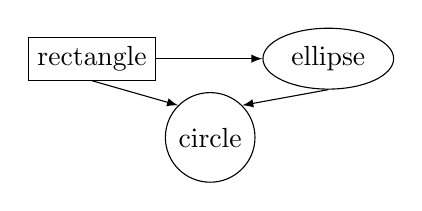
\begin{tikzpicture}
	\node (r) at (0,1) [draw, rectangle] {rectangle};
	\node (c) at (1.5,0) [draw, circle] {circle};
	\node (e) at (3,1) [draw, ellipse] {ellipse};
	\draw [-latex] (r.east) -- (e.west);
	\draw [-latex] (r.south) -- (c.north west);
	\draw [-latex] (e.south) -- (c.north east);
\end{tikzpicture}



\begin{tikzpicture}
	\node [graduate, monitor, minimum size=2cm] (student) {};
	\node at (student.45) [starburst, draw=red, fill=yellow,
		starburst point height=0.4cm, line width=1pt,
		font=\ttfamily\scriptsize, inner sep=1.5pt] {error};

	\node at (student.130) [cloud callout, cloud puffs=13,
		aspect=3, anchor=pointer, shading=ball,
		ball color=darkgray, text=white, font=\bfseries] {My thesis...!};
\end{tikzpicture}


\end{document}
